%! Author = alida
%! Date = 20/11/2024

% Preamble
\documentclass[@SRC@/main]{subfiles}

\graphicspath{{@IMAGES@}}
% tutti i pacchetti usati vanno nel main

% Document
\begin{document}
\clearpage
\section{Analisi}
Le misure di calibrazione confermano il corretto funzionamento degli
strumenti.
\begin{center}
\begin{minipage}{.8\textwidth}
  \centering
  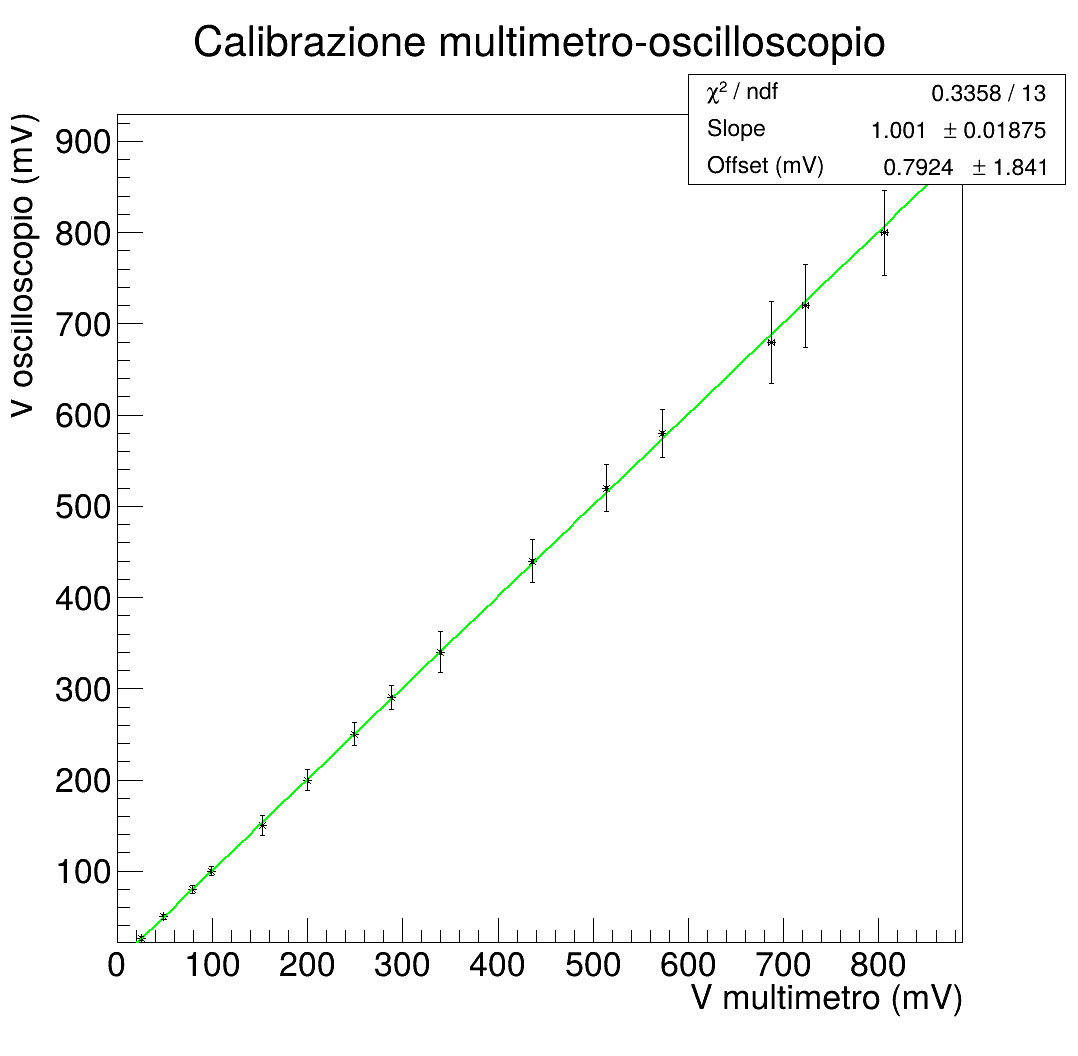
\includegraphics[width=.75\textwidth]{calibrazione.png} 
  \captionof{figure}{Grafico e fit dei valori ottenuti dalla misura di calibrazione}
  \label{fig:calibrazione}
\end{minipage}
\end{center}
\vspace{.25cm}
Il fit lineare sui dati in Tabella~\ref{tab:calibrazione}
(Figura~\ref{fig:calibrazione}) fornisce i seguenti valori:
\begin{center}
\begin{minipage}{.95\textwidth}
  \centering
  \begin{tabular}{||c|c||}
    \hline
    Pendenza & Intercetta (mV) \\
    \hline
    $1.001 \pm 0.019$ & $0.8 \pm 1.8$ \\
    \hline
  \end{tabular}
  \captionof{table}{Risultati del fit sui dati di calibrazione}
  \label{tab:fit-calibrazione}
\end{minipage}
\end{center}
Come si può vedere in Tabella~\ref{tab:fit-calibrazione} entrambi i risultati
sono compatibili con i valori attesi entro gli errori: rispettivamente 1 e 0. \\

I dati delle curve caratteristiche (Tabelle~\ref{tab:silicio}~e~\ref{tab:germanio}) sono
fittati secondo l'eq\,\eqref{eq:caratteristiche} ma anche in scala semi logaritmica dove la
relazione diventa:
\begin{equation*}
  \ln (I(V_D)) = \ln \left( I_0 \cdot \exp^{\frac{V_D}{\eta V_T}} \right) \implies
  I_{ln}(V_D) = \frac{1}{\eta V_T} \cdot V_D + \ln (I_0)
\end{equation*}
Questa relazione permette di utilizzare la regrssione lineare, generalmente
più precisa del genrico metodo del minimo $\chi^2$; si veda
l'appendice~\ref{subsec:propagazione-errori-log} per la propagazione degli
errori in scala semi logaritmica.
\begin{center}
\begin{minipage}{.95\textwidth}
  \centering
  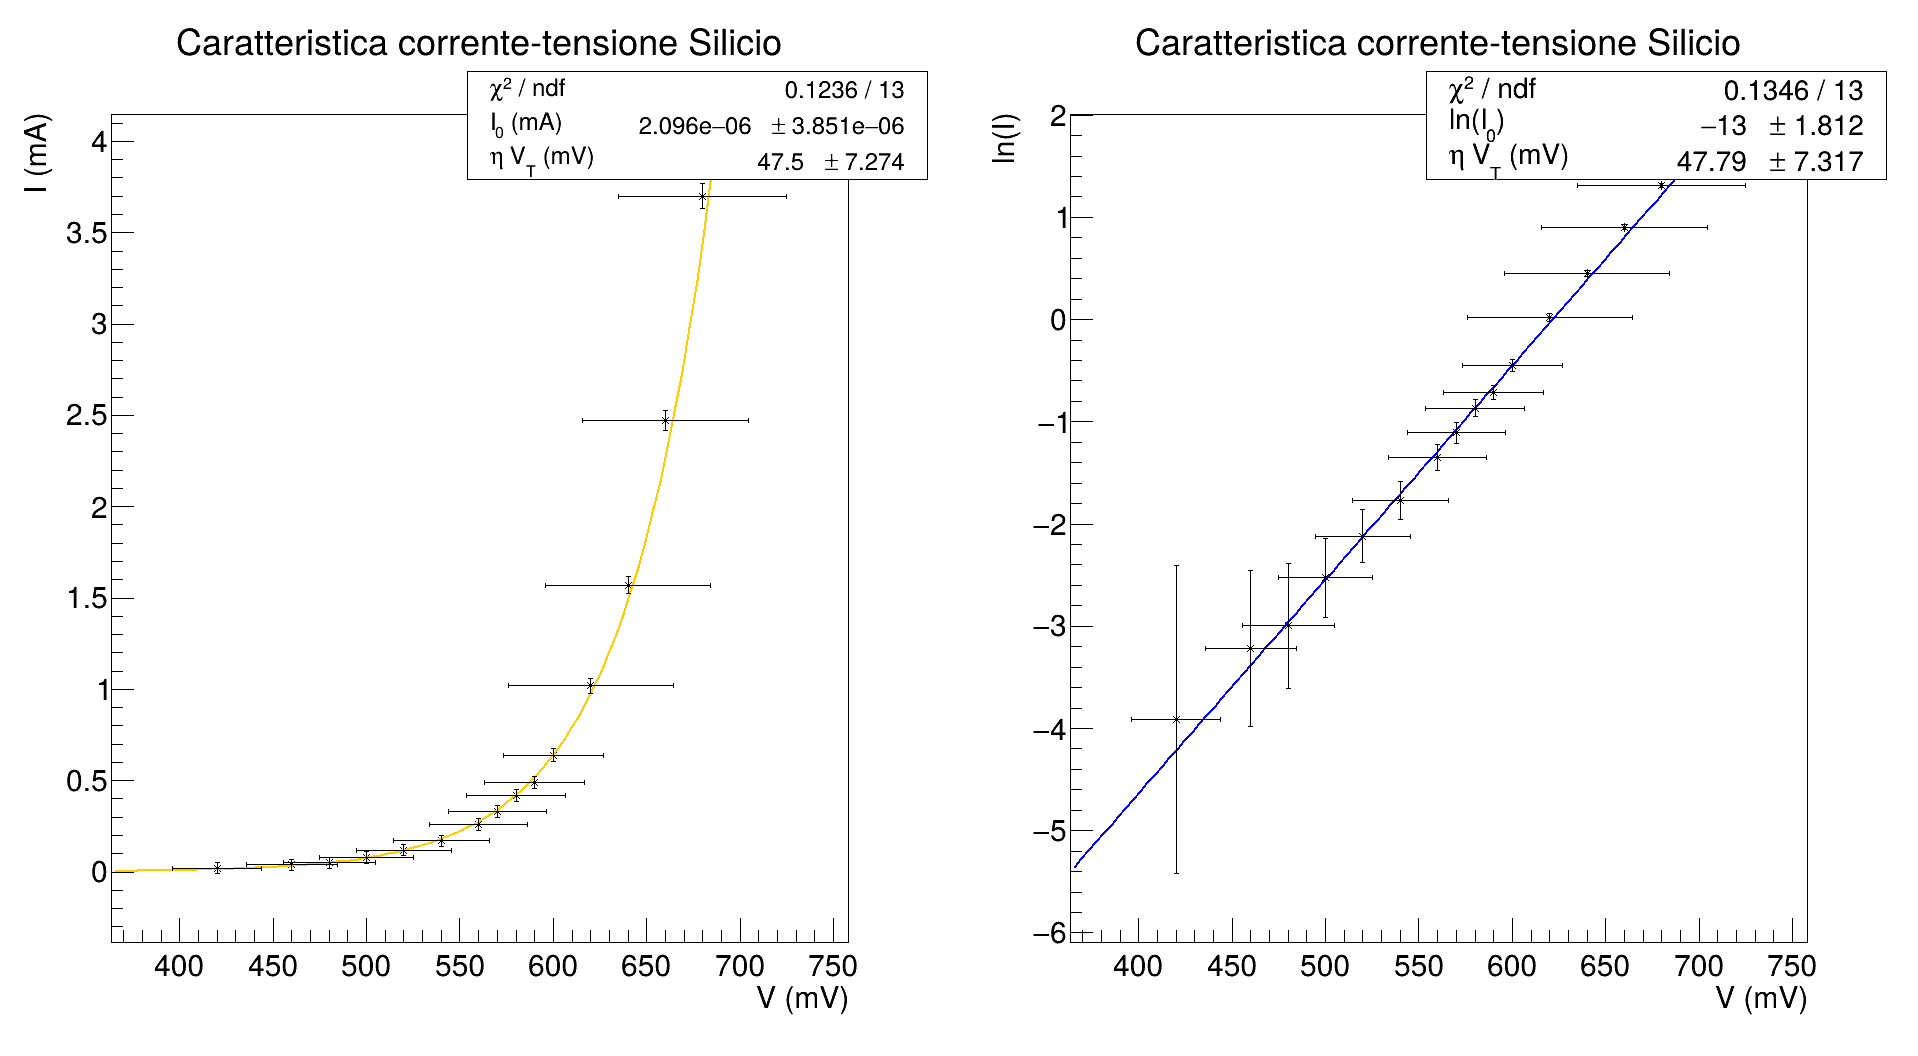
\includegraphics[width=\textwidth]{silicio.png}
  \captionof{figure}{schematizzazione della struttura del disco, nella prima figura visto dall'alto, nella seconda met\`a di una sezione frontale.}
  \label{fig:silicio}
\end{minipage}
\\
\begin{minipage}{.95\textwidth}
  \centering
  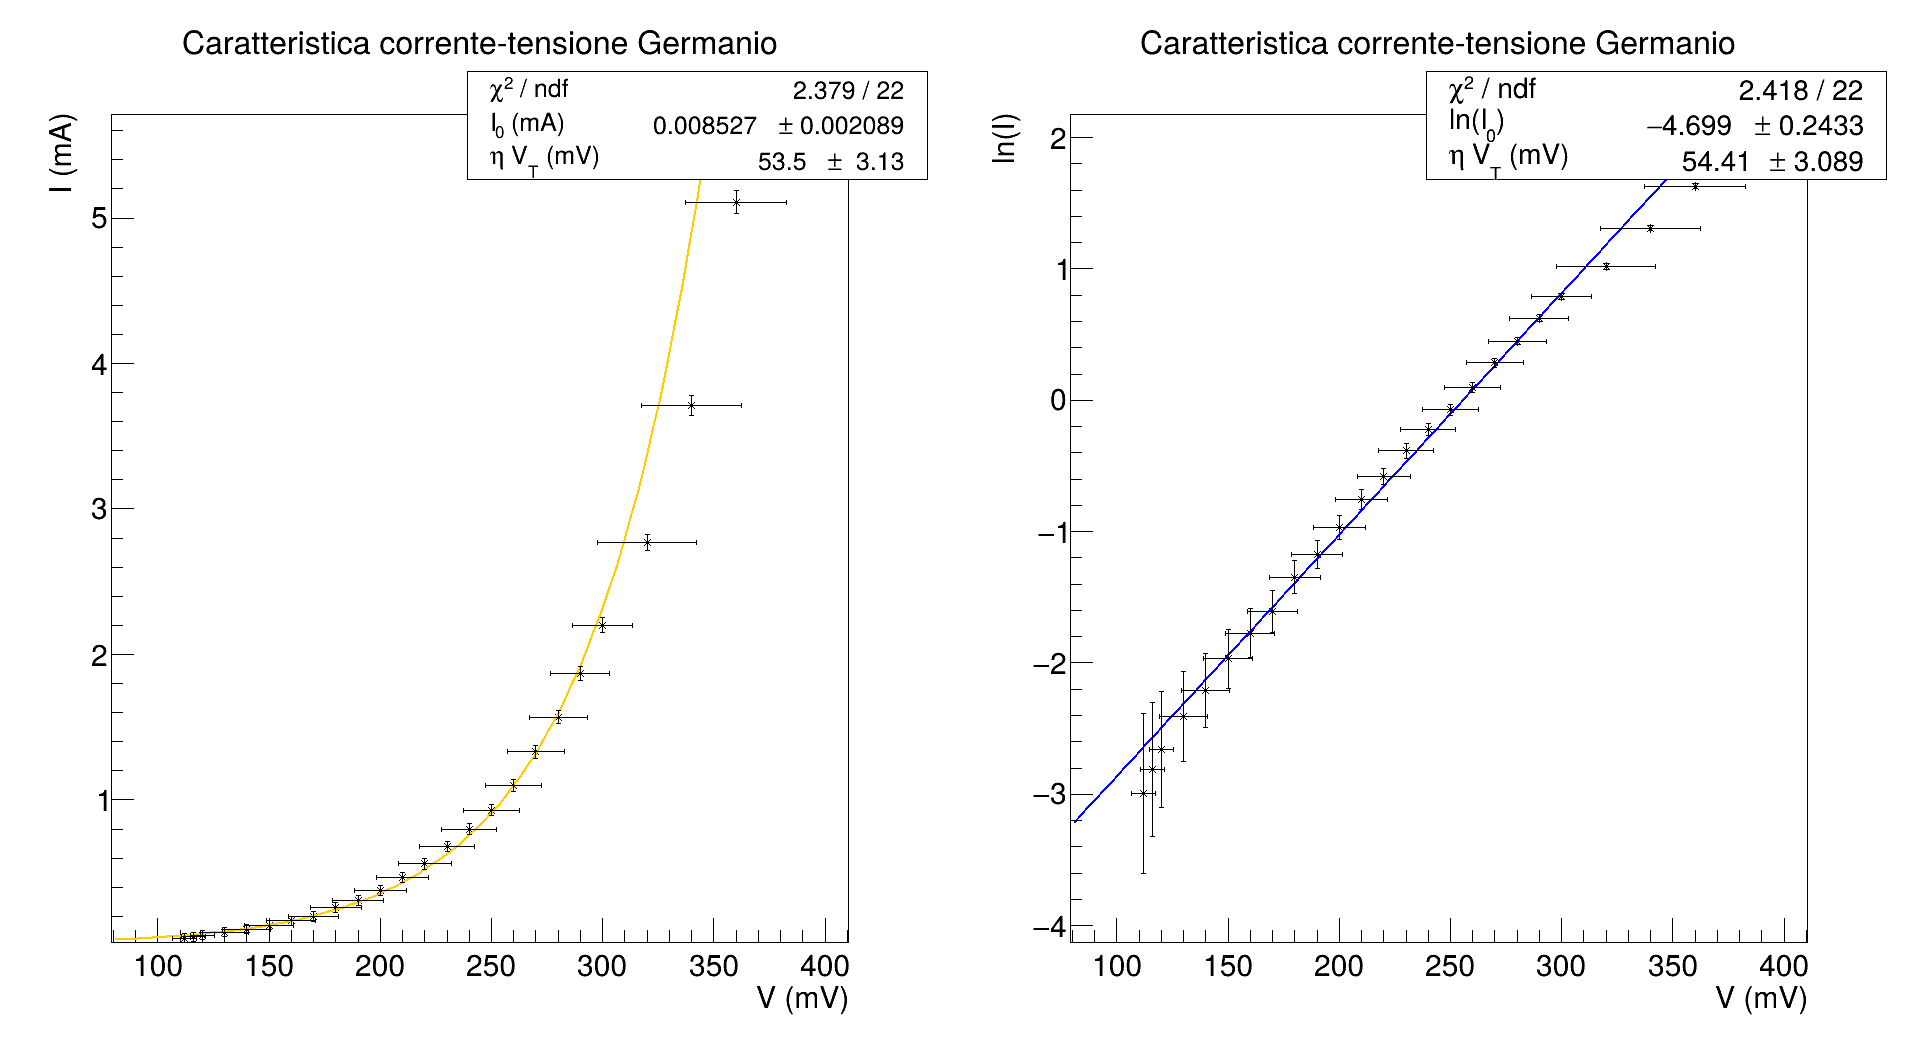
\includegraphics[width=\textwidth]{germanio.png}
  \captionof{figure}{schematizzazione della struttura del disco, nella prima figura visto dall'alto, nella seconda met\`a di una sezione frontale.}
  \label{fig:germanio}
\end{minipage}
\end{center}
I risultati dei fit nelle Figure \ref{fig:silicio} e \ref{fig:germanio}, sono:
\begin{table}
  \centering
  \begin{subtable}{.45\textwidth}
    \centering
    \begin{tabular}{||c|c|c||}
      \hline
      \multicolumn{3}{||c||}{Silicio} \\
      \hline
      Scala & $\eta V_T$ & $I_0$ \\
      \hline
      lineare & & \\
      \hline
      semi logaritmica & & \\
      \hline
    \end{tabular}
    \caption{Risultati fit caratteristica diodo al silicio}
    \label{tab:fit-silicio}
  \end{subtable}
  \hfill
  \begin{subtable}{.45\textwidth}
    \centering
    \begin{tabular}{||c|c|c||}
      \hline
      \multicolumn{3}{||c||}{Germanio} \\
      \hline
      Scala & $\eta V_T$ & $I_0$ \\
      \hline
      lineare & & \\
      \hline
      semi logaritmica & & \\
      \hline
    \end{tabular}
    \caption{Risultati fit caratteristica diodo al germanio}
    \label{tab:fit-germanio}
  \end{subtable}
  \caption{Risultati dei fit sui dati delle caratteristiche dei due diodi}
  \label{tab:fit-diodi]
\end{table}

Entrambi i fit restituiscono risultati compatibili entro gli errori.

\end{document}